\documentclass[../../lectures.tex]{subfiles}

\begin{document}

\chapter{Файловые системы}

\section{Носители}
\subsection{HDD}
\centerimage{hard-disk.jpg}{Жесткий диск}{1}
\begin{itemize}
    \item Обороты в минуту($O$) --- 5400, 7200, 10000, ...
    \item $~\frac{1}{2 * O}$ --- минимальное время доступа (случайное чтение)
    \item В мире Unix не существует дефрагментации (ОС должна сама заботиться)
    \item Время отказа (\textbf{MTBF} --- min time before failure) --- условное 
          количество циклов наработки до отказа
    \item На server --- сутки, desktop --- часы (разница в 3 раза примерно, 
          если одно и то же число циклов)
    \item Плюсы: стоимость, объем
    \item Минусы: время доступа, надежность
\end{itemize}

\subsection{Общее}
\begin{itemize}
    \item \textbf{EOPS} --- \todo{}
    \item \textbf{seek} --- рандомное чтение (512 байт)
    \item \textbf{SATA} и \textbf{NVME} --- протоколы для дисков
    \item \textbf{NVME} --- новомодная штука для \textbf{SSD}
    \item Минимум информации: сектор --- 512 байт -> 4096 байт
    \item Чтение одного байта равносильно чтению всего сектора с этим байтом
    \item Запись одного байта --- считать один сектор, заменить байт и записать один сектор
    \item Аналогия --- процессор-память --- \textbf{cacheline}
\end{itemize}

\section{Быстродействие}
\subsection{Интересные числа}
\begin{center}
Числа, которые должен знать каждый программист
\begin{tabular}{| l | l |}
    \hline
    Cycle                            & 1   ns \\ \hline
    Main memory reference            & 100 ns \\ \hline
    Read 4K randomly from SSD        & 150 us \\ \hline
    Read 1 MB sequentially from SSD  & 1   ms \\ \hline
    Disk seek                        & 10  ms \\ \hline
    Read 1 MB sequentially from disk & 20  ms \\ \hline
\end{tabular}
\end{center}
\subsection{Выводы для HDD}
\begin{itemize}
    \item Читать нужно последовательно
    \item Обращения к диску следует минимизировать
    \item Стоимость доступа сильно дороже передачи данных
\end{itemize}

\section{Structure packaging}
Сколько будет занимать памяти следующая структура?

\code{hole1.c}{C}

Ответ: 32 байта, так как $b$ и $d$ будут выравнены по MAX\_ALLIGNMENT

Очевидное решение проблемы:

\code{hole2.c}{C}

Данная структура будет занимать 24 байта на x86\_64.

\section{Алгоритмы элеватора}
\textcolor{blue}{\href{https://slideplayer.com/slide/5209336}{Ссылка на презентацию}}
\begin{enumerate}
    \item SLIDE 6
        
          Алгоритмы элеватора обрабатывают последовательности запросов к диску (переупорядочивают их)
    \item SLIDE 7

          \textbf{FCFS} (FIFO) --- самый простой и медленный
    \item SLIDE 8-9

          \textbf{SSTF} (Shortest Seek Time First)--- сортировка (очередной запрос определяется наименьшим временем seek)
    \item SLIDE 10 - \dots

          Различные способы упорядочивания(\textbf{SCAN})
\end{enumerate}

\section{Файл}
\begin{itemize}
    \item Абстракция для данных
    \item Последовательность байтов
    \item Формат не определен
    \item \textbf{Unix} --- все есть файл (абстракция-интерфейс внутри ядра)
    \item Типы файлов 
          \begin{itemize}
            \item regular
            \item directory
            \item symlink
            \item socket, fifo
            \item character device, block device
          \end{itemize}
\end{itemize}

\section{Директория}
\begin{itemize}
    \item Содержит имена находящихся в ней файлов
    \item $.$ --- ссылка на текущую
    \item $..$ --- ссылка на родителя
    \item \shell{cd}, \shell{pwd}
    \item Формирование дерева: \shell{ls}
    \item \shell{find} --- поиск
    \item \emph{filename vs pathname}: \shell{realpath}
\end{itemize}
\subsection{Права --- просто числа}
\begin{itemize}
    \item \shell{view /etc/passwd}
    \item \shell{view /etc/group}
    \item \shell{id} - показывает идентификаторы того, кто ее вызывал
    \item \shell{execute} --- search
    \item \shell{read} --- directory listing
    \item \shell{write} --- changing directory
    \item Темные директории (переход в директорию внутри директории, для который ты не можешь посмотреть все файлы)
    \item Права rwx (read, write, execute)
    \item \shell{chmod} --- меняет права доступа
          
          \shell{chmod 123} --- 1 - user, 2 - group, 3 - other
    \item У процесса есть информация о том, кто его запустил
\end{itemize}
\subsection{sticky bit}
\begin{itemize}
    \item Изменение поведения при создании нового файла
    \item /tmp
    \item Создаешь директорию со \emph{sticky bit} и все, кто создают файлы в этой директории имеют на них права
\end{itemize}

\section{Иерархия}
\begin{itemize}
    \item $/$
        \begin{itemize}
            \item bin/
            \item dev/
            \item etc/
            \item sbin/
            \item home/
            \item var/
            \item usr/
                \begin{itemize}
                    \item bin/
                    \item sbin/
                \end{itemize}
            \item tmp
        \end{itemize}
\end{itemize}

\section{Монтирование}
\begin{itemize}
    \item Есть корень и есть узлы, в которые можно монтировать другие файловые системы (часть из них виртуальная)
    \item \shell{mount}
    \item Для $/$ обычно используется \textbf{ext4} (использует журналирование)
    \item Для /boot может использоваться \textbf{ext2} --- так как это более проверено временем (на Ubuntu)
    \item Файловая система для узла --- это не константа, ее можно менять
    \item \shell{df - h}, \shell{du -hs}
\end{itemize}

\section{Inode}
\todo{More from presentation}
\begin{itemize}
    \item Директория задает mapping имени файла в его inode
    \item \shell{ln}
    \item Hardlink --- существует в рамках одной файловой системы
    \item Softlink(symlink) --- бит l
    \item \shell{stat} --- информация о файле
    \item \emph{atime} --- время последнего доступа
    \item \emph{ctime} --- изменение мета-информации
    \item \emph{mtime}--- изменение содержимого файла
\end{itemize}

\section{Атрибуты процесса}
\todo{}

\section{Файловые процессы}
\todo{}

\section{Диски}
\centerimage{disk-mechanism.jpg}{Устройство диска}{1}
\todo{Информация из презентации}
\begin{itemize}
    \item На внешних цилиндрах больше секторов, чем на внутренних 
          => чем ближе к центру тем меньше скорость нужна (CD)
    \item На жестких дисках --- постоянная угловая скорость 
          (в центре больше плотность)
    \item \emph{Partitioning} --- разделение диска на несколько 
          логических частей (партиции, на каждой своя файловая система)
    \item Существует другой подход - "собственная" файловая система 
          на "сыром" диске (MySQL)
    \item Современный контроллер жесткого диска может находить механически поврежденные блоки (bad blocks) и делать remap их на некоторые запасные (sector sparing: replace bad sectors with spare)
    \item \shell{man 1 badblocks}
    \item Bootblock --- \todo{}
\end{itemize}

\section{RAID}
Redundant Arrays of Independent Disks (Избыточный массив независимых дисков)
\centerimage{raid-levels.jpg}{Уровни RAID}{1}
\begin{itemize}
    \item Reilability (надежность, hacks for more long time of complex usage)
    \item Perfomance (striping, суммирование EOPS)
    \item Levels:
        \begin{itemize}
            \item 0 --- pure striping (1 блок на 1 диске, 2 блок на 2 диске и т.д. --- один диск вышел из строя --- fail)
            \item 1 --- pure mirroring (пара дисков, данные продублированы)
            \item 0 + 1, 1 + 0
            \item 2, 3, 4, 5 --- используются не так часто (хранение доп. данных)
        \end{itemize}
    \item Rebuild --- падает производительность
    \item Hardware RAID --- проблемы: "залоченность" на производителе (vendor lock in), драйвера, как правило, не очень
    \item Software RAID --- гипотетически медленно, но на практике нужная производительность достигается
    \item У аппаратных RAID --- есть батарейка, которая "улучшает" производительность 
          (сначала на батарейку, потом на диск, когда будет удобно)
\end{itemize}

\section{Организация файловых систем}
Структура директорий: связный список и хэш-таблица

smart (\shell{smartctl}) --- оценка диска на практике

Свободные сектора
\begin{enumerate}
    \item Bit Vector --- fast, space usage
    \item Список
\end{enumerate}

\begin{center}Выделение памяти\end{center}

\begin{figure}[H]
\captionsetup{singlelinecheck=off}
\begin{minipage}[c]{0.5\linewidth}
\centering
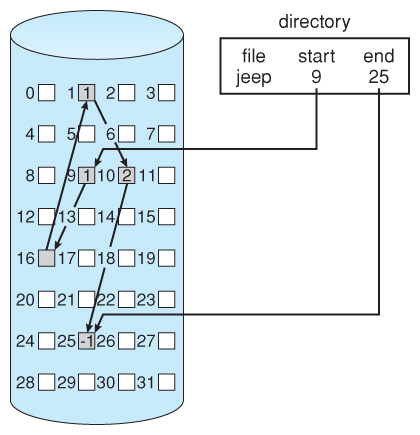
\includegraphics[width=\textwidth]{images/linked-allocation.jpg}
\end{minipage}
\hspace{0.5cm}
\begin{minipage}[c]{0.5\linewidth}
\centering
Линейное
\begin{itemize}
    \item Объект задается началом и концом (здесь возникают проблемы внешней и внутренней фрагментации)
    \item Perfomance: +sequential, +random
\end{itemize}
\end{minipage}
\end{figure}

\begin{figure}[H]
\captionsetup{singlelinecheck=off}
\begin{minipage}[c]{0.5\linewidth}
\centering
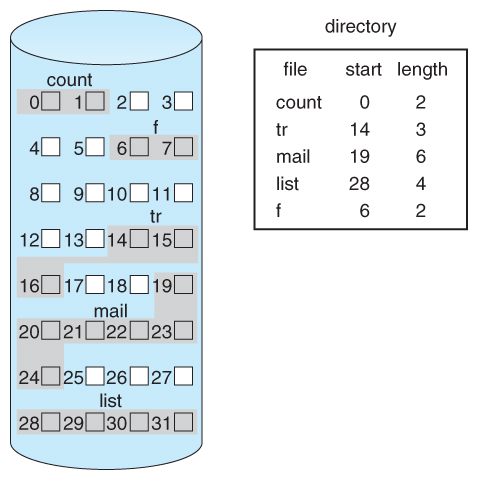
\includegraphics[width=\textwidth]{images/contiguous-allocation.jpg}
\end{minipage}
\hspace{0.5cm}
\begin{minipage}[c]{0.5\linewidth}
\centering
Список
\begin{itemize}
    \item Perfomance: -sequential, --random
    \item Надежность: -
    \item Решает проблему внешней фрагментации
    \item В каждом "блоке" указатель на следующий
\end{itemize}
\end{minipage}
\end{figure}

\begin{figure}[H]
\captionsetup{singlelinecheck=off}
\begin{minipage}[c]{0.5\linewidth}
\centering
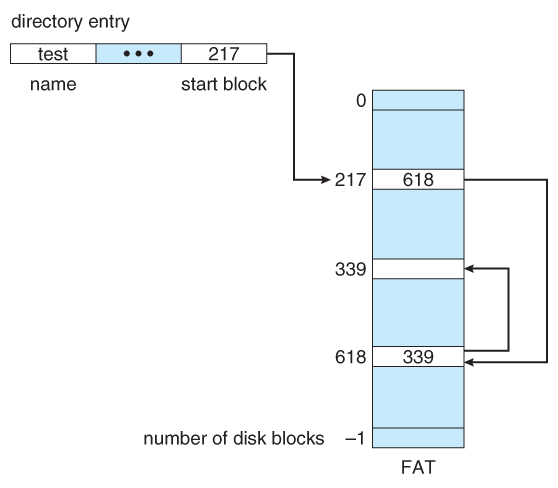
\includegraphics[width=\textwidth]{images/fat-table.jpg}
\end{minipage}
\hspace{0.5cm}
\begin{minipage}[c]{0.5\linewidth}
\centering
FAT
\begin{itemize}
    \item Все ссылки хранятся в начале диска --- их можно эффективно кэшировать
\end{itemize}
\end{minipage}
\end{figure}

\begin{figure}[H]
\captionsetup{singlelinecheck=off}
\begin{minipage}[c]{0.5\linewidth}
\centering
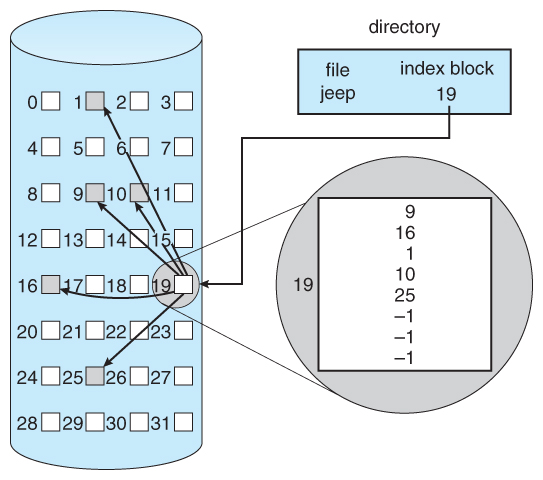
\includegraphics[width=\textwidth]{images/indexed-allocation.jpg}
\end{minipage}
\hspace{0.5cm}
\begin{minipage}[c]{0.5\linewidth}
\centering
Индексированная
\begin{itemize}
    \item Отдельный блок для ссылок на данные
    \item Внутренняя фрагментация
\end{itemize}
\end{minipage}
\end{figure}

\begin{figure}[H]
\captionsetup{singlelinecheck=off}
\begin{minipage}[c]{0.5\linewidth}
\centering
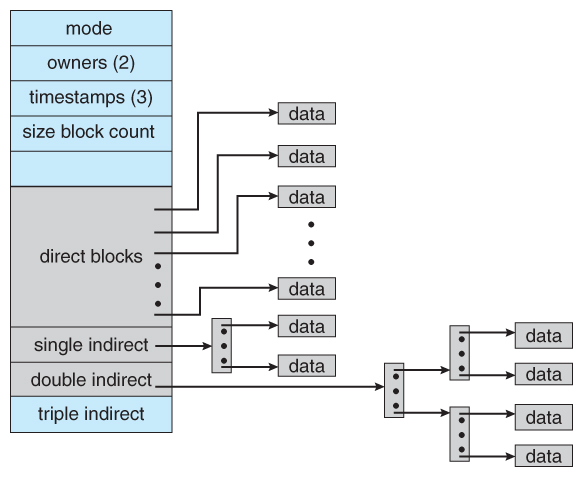
\includegraphics[width=\textwidth]{images/unix-inode.jpg}
\end{minipage}
\hspace{0.5cm}
\begin{minipage}[c]{0.5\linewidth}
\centering
UNIX
\begin{itemize}
    \item Комбинированная
    \item Косвенная многоуровневая адресация
\end{itemize}
\end{minipage}
\end{figure}

\section{Операции с файлами}
\todo{3 картинки + презентация}

\section{Системные вызовы}

\section{Пару слов о типах}

\section{Common pitfalls}

\section{Литература}
\begin{itemize}
    \item The Unix Programming Environment. Brian W. Kernighan, Rob Pike
    \item Advanced Programming in the Unix Environment. W. Richard Stevens
\end{itemize}

\section{Домашнее задание №2}
\end{document}
